\documentclass{article}
\usepackage{geometry}
\geometry{a4paper}
\usepackage{amsmath}
\usepackage{empheq}
\usepackage{mhchem} % Package for chemical equation typesetting
\usepackage{siunitx} % Provides the \SI{}{} command for typesetting SI units
\usepackage{parskip}
\usepackage{graphicx} % Required for the inclusion of images
\usepackage{amssymb}
\usepackage{placeins}
\usepackage{cancel}
\usepackage{fullpage}
%\usepackage{subfig}
\usepackage{enumitem}
\usepackage{listings}
%\usepackage{mcode}
\usepackage{wrapfig}
%\renewcommand{\labelenumii}{\alph{enumi}.}
%Alph for uppcer case, \arabic for 1, 2, 3
%\roman for i, ii, iii \alph{enumi})
% Make numbering in the enumerate environment by letter rather than number (e.g. section 6)
\usepackage{booktabs, multicol, multirow}
%\usepackage[ ]{mcode} 

\setlength\parindent{0pt} % Removes all indentation from paragraphs

\renewcommand{\labelenumi}{\alph{enumi}.} % Make numbering in the enumerate environment by letter rather than number (e.g. section 6)

%\usepackage{times} % Uncomment to use the Times New Roman font

\include{paulsmacros}
%\braces , \parens \brackets \mC (matrix C) \vv (vector v) \h hats for somethings ie \hvy or \hmA \sA (subscript upper case)
\usepackage{caption}
\usepackage{subcaption}

%----------------------------------------------------------------------------------------
%	DOCUMENT INFORMATION
%----------------------------------------------------------------------------------------
%$\frac{-1}{\sqrt{a}}$
%\title{Newberry/Felix  \hfill \today}
%\date{}
\begin{document}
%\maketitle 
%\LARGE
\textsc{\Large Structure Solver Validation \hfill \today}\\[0.5cm] % Name of your university/college
\textsc{\large Felix Newberry}\\

This report details the  validation of a nonlinear dynamic solver that utilizes Fenics  through comparison to benchmark computations. The solver is found to be accurate. The code in question can be found in the Github repository under \verb|/4_Structure_test/Turek_benchmark/structure_dynamic_fenics.py|


\section{Problem Setup} 

The nonlinear dynamic structure problem is solved in Fenics with the $CG_1$ method \cite{eriksson1996computational}. The method is described in chapter 27 of the Fenics book that addresses nonlinear elasticity \cite{logg2012automated}. Speicifically, 27.2.3 details time-stepping algorithims for nonlinear elastic models. The structure solver was validated with the structure test case of an elastic beam attatched to a cylinder \cite{turek2006proposal}. Only the dynamic solver is addressed in this report. 

\subsection{Geometry}
The geometry of the problem is depicted in Figure \ref{fig:geom}. 

\FloatBarrier
\begin{figure}[h]
\centering
	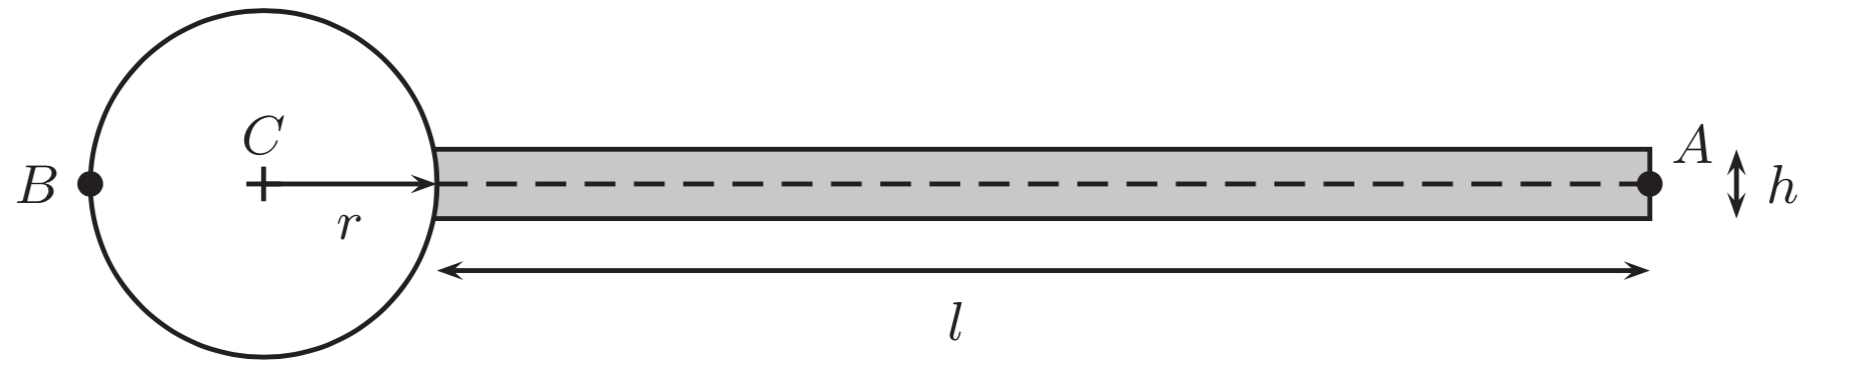
\includegraphics[width=\textwidth]{struct_geom}
	\caption{Structure geometry \cite{turek2006proposal}}
	\label{fig:geom}
\end{figure}
\FloatBarrier

An elastic bar of length $l = 0.35 m$ and height $ h = 0.02 m$ is attached to circular cylinder of diameter $D = 0.1 m$. The left end of the is fully attached to the cylinder. This benchmark is designed to test the structure component of a fluid structure interaction (FSI) problem. 

\subsection{Boundary Conditions}
The left end of the bar is fixed to the cylinder. The traction on the bar surface is set to zero. A gravitational force of $ \textbf{g} = (0, 2) $ is applied to the elastic bar. 

\subsection{Structure Properties}
The structure is modeled as elastic and compressible. The material is St. Venant-Kirchhoff. The first lame constant was defined as $\mu = 0.05 kg m^{-1}s^{-2}$, the Poisson ratio as $\nu = 0.4$ and the density as $\rho = 1000 kg m^{-3}$.

\subsection{Validation Metrics}

The metric for validation is the x and y deflection of monitor point A, depicted in Figure \ref{fig:geom}. The benchmark provids data for both static and dynamic tests, though only the dynamic results are utilized in this report \cite{turek2006proposal}. The benchmark states that the mean and amplitude of the deflection is computed from the last period of the oscillations. Problematically, the duration of the simulation is not specified. For the purposes of this report it is assumed to be 10 s which is the size of the window Figure \ref{fig:CSM_1}  calculating the mean and max values and from these and computing the mean as the average of these values and the amplitude as half the difference:

\begin{equation}
mean = \frac{1}{2}(max + min)
\end{equation}

\begin{equation}
amplitude = \frac{1}{2}(max - min)
\end{equation}

Two alternatives of oscillation frequency measurement are suggested in the benchmark. The first is to measure the  period T and compute the frequency as

\begin{equation}
frequency = \frac{1}{T}
\end{equation}

The second is to use Fourier analysis on the data. In this report the frequency was calculated from the average period of 10 oscillations. 

\section{Validation} 

The x and y deflection of point A is plotted against time in Figures \ref{fig:CSM_1} and \ref{fig:CSM_2} for the benchmark and calculated data respectively. 

\begin{figure}[h]
\centering
	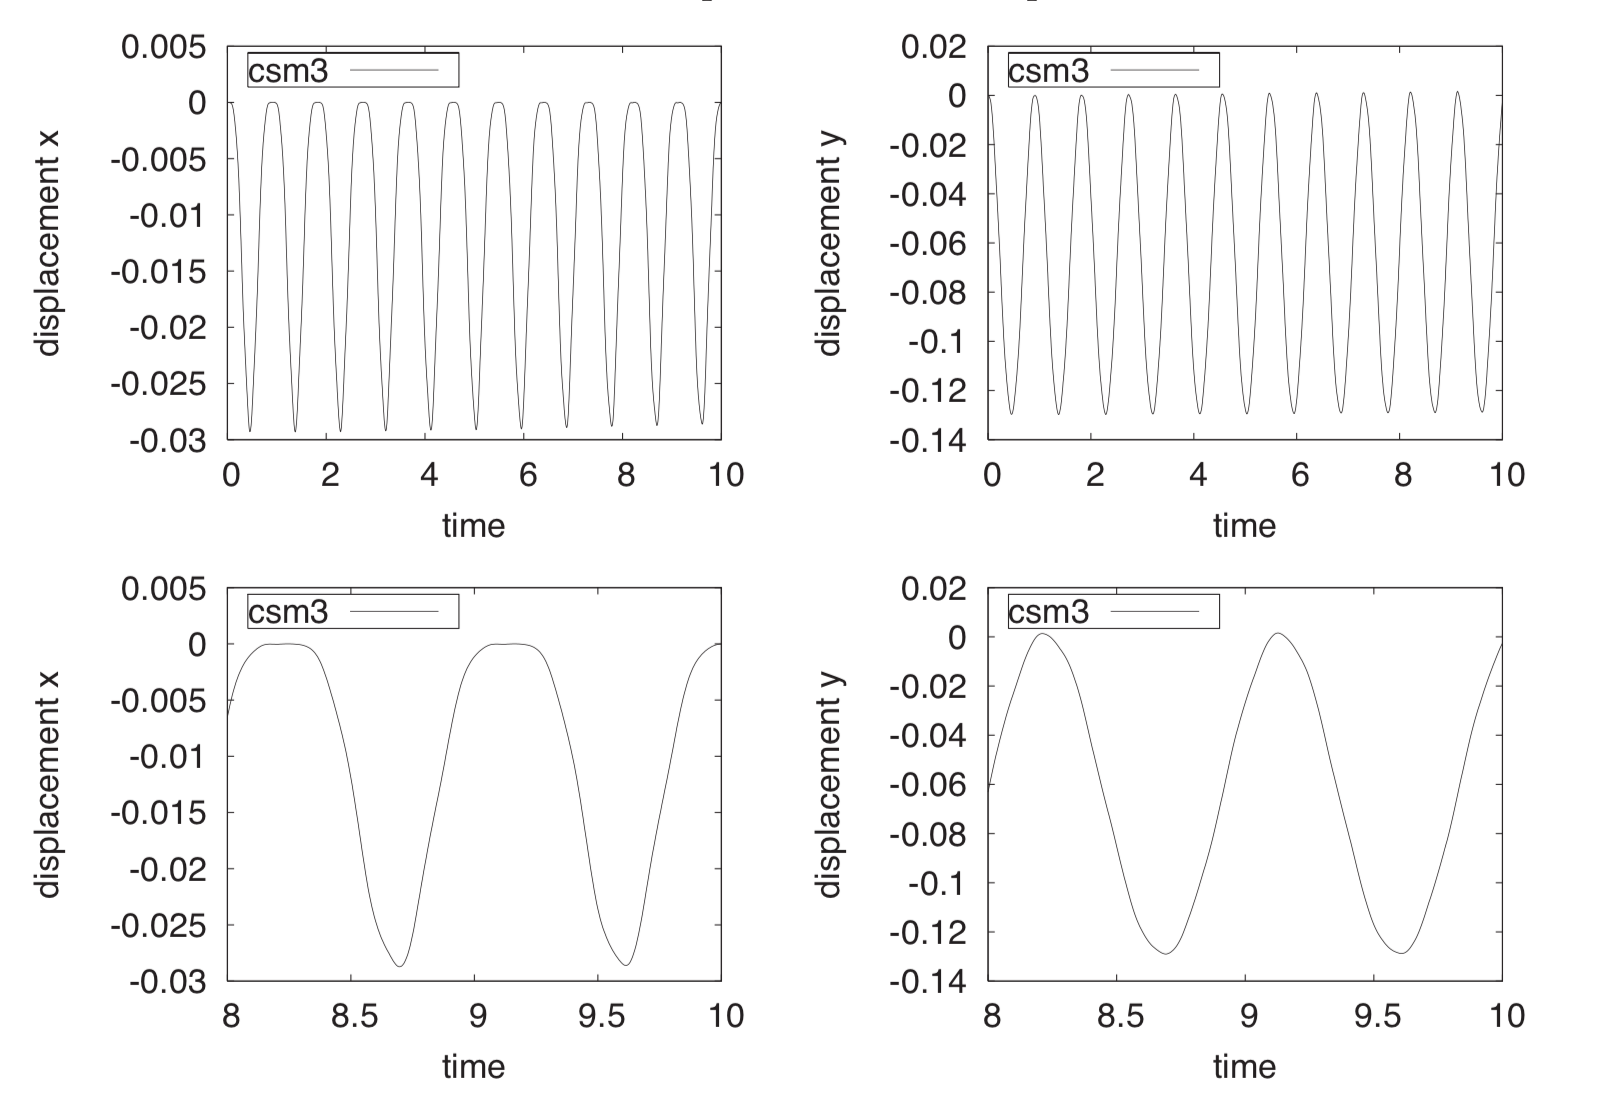
\includegraphics[width=0.6\textwidth]{CSM_1}
	\caption{Displacement of point A benchmark data \cite{turek2006proposal}}
	\label{fig:CSM_1}
\end{figure}

\begin{figure}[h]
\centering
	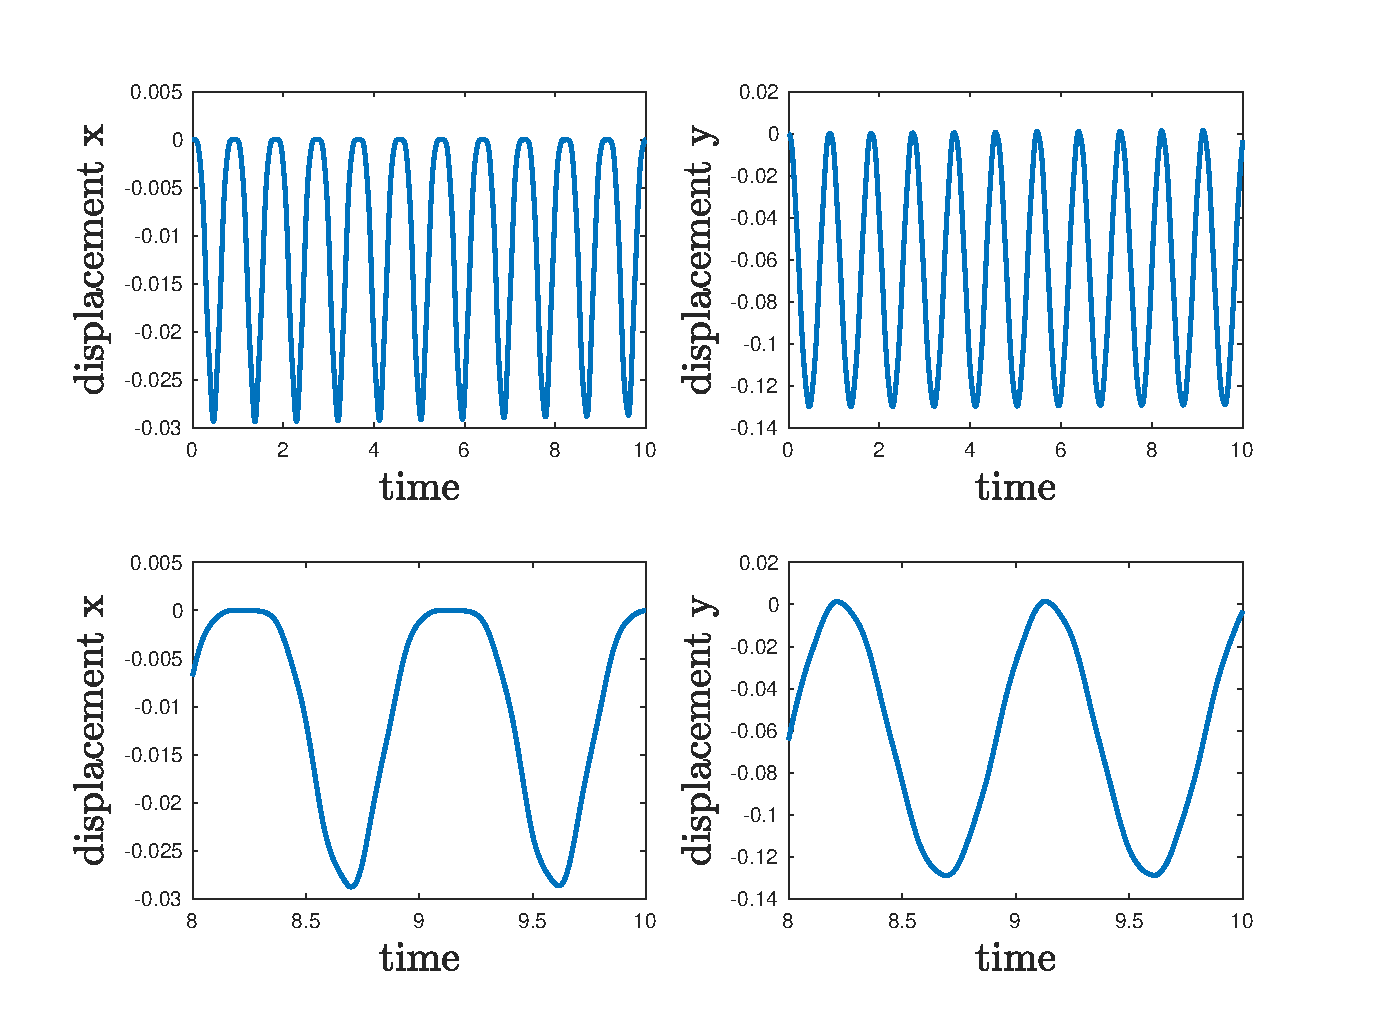
\includegraphics[width=0.6\textwidth]{CSM_2}
	\caption{Simulated displacement of point A}
	\label{fig:CSM_2}
\end{figure}


Evident in Figures \ref{fig:CSM_1} and \ref{fig:CSM_2} is a clear alignment in dynamic behavior of the benchmark and the test data. By eye there is no discernible difference. This assertion is compounded by comparison to the benchmark data presented in Figure \ref{fig:CSM_3}.

\FloatBarrier
\begin{figure}[h]
\centering
	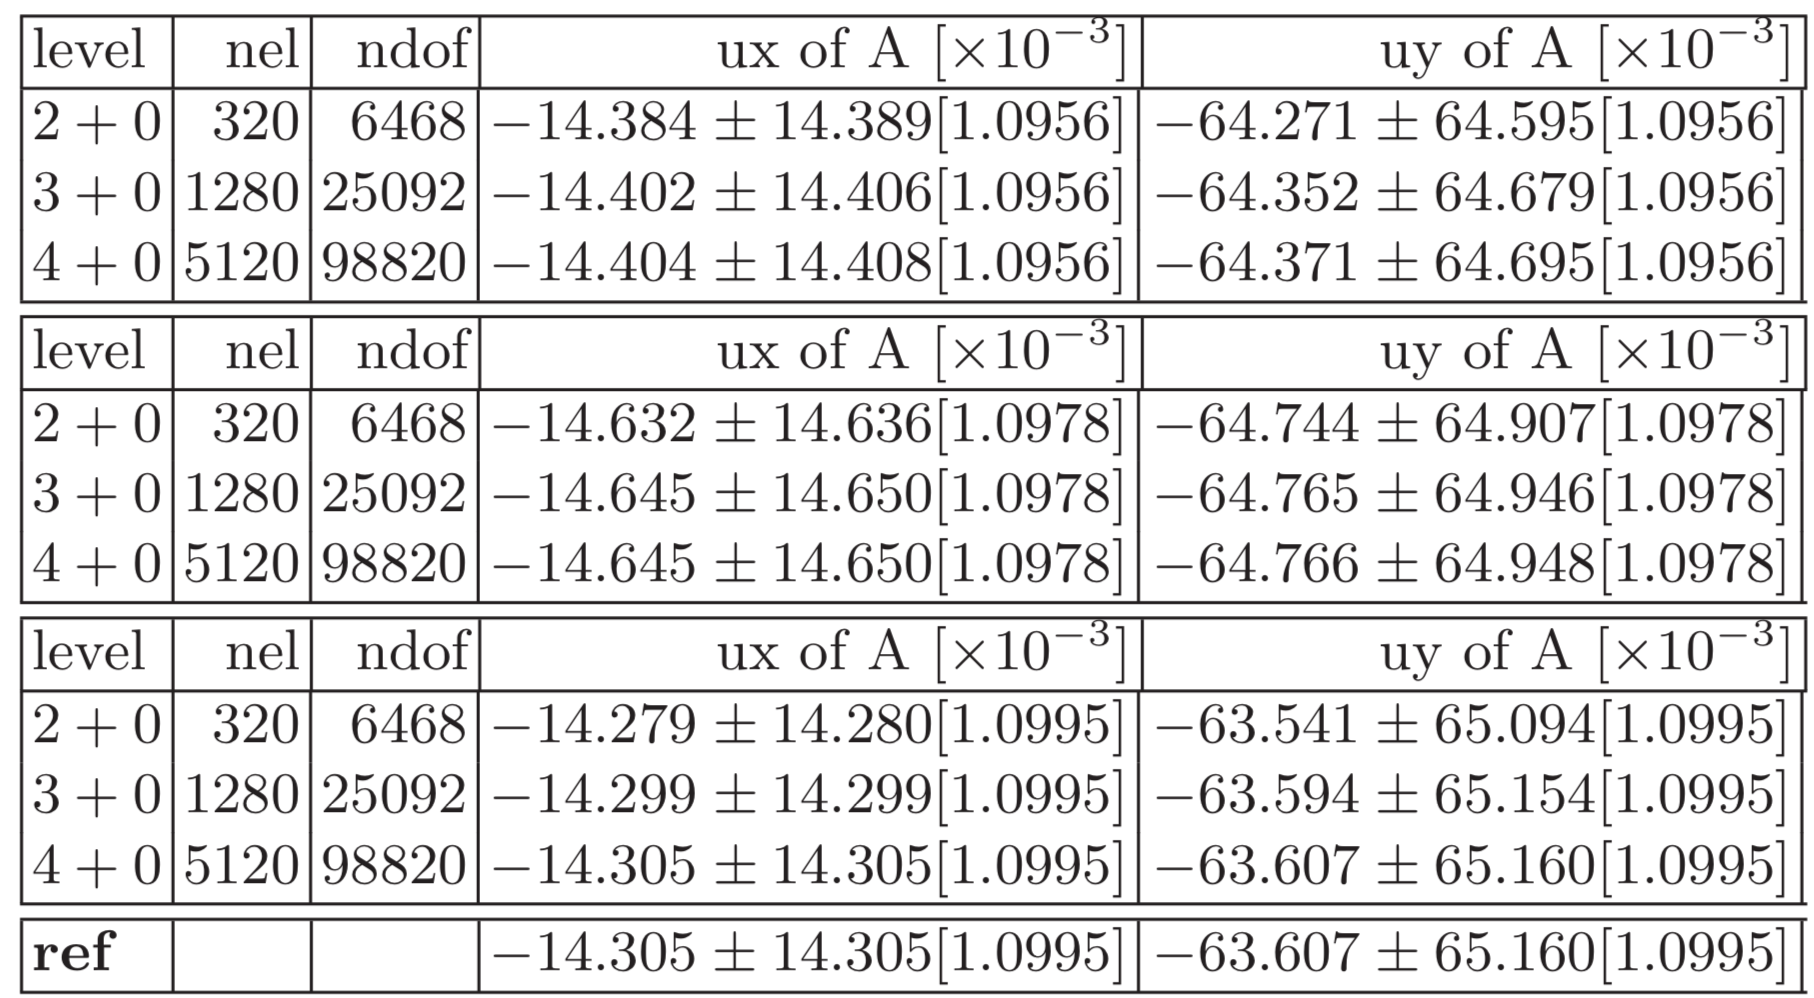
\includegraphics[width=0.6\textwidth]{CSM_3_data}
	\caption{Benchmark dynamic solutions for with timesteps of $dt = 0.02$, $0.01$, $0.005$ \cite{turek2006proposal}}
	\label{fig:CSM_3}
\end{figure}

Table \ref{tab:struct} presents the simulated results for comparison. Simulations were run with similar values of ndof to the benchmark. The results of Table \ref{tab:struct} were computed from an interval of $T = 10 s$. 

\FloatBarrier
  \begin{table}[htbp]
  \setlength\extrarowheight{5pt}
  \centering
  \caption{Results for dynamic test case with time steps $dt = 0.02$, $0.01$, $0.005$}
    \begin{tabular}{ccc}
    \toprule
     ndof & ux of A $[\times 10^{-3}]$ & uy of A $[\times 10^{-3}]$ \\
    \midrule
7906 & $-14.379 \pm 14.400 [1.0949]$ & $-64.438 \pm 64.578[1.0949] $\\
29850 & $-14.383 \pm 14.407 [1.0949] $ & $-64.445 \pm 65.593 [1.0949] $\\
105134 & $-14.379 \pm 14.400[1.0949]  $ & $-64.438 \pm 64.578[1.0949]  $\\
    \midrule
7906 & $-14.464 \pm 14.465 [1.0941] $ & $-64.787\pm 64.971 [1.0941]$\\
29850 & $-14.673 \pm 14.679 [1.0941]$ & $-64.841 \pm 65.025 [1.0941]$\\
105134 & $-14.665 \pm 14.672 [1.0941] $ & $-64.826 \pm 65.010 [1.0941] $\\
    \midrule
7906 & $-14.311 \pm 14.311 [1.0917]$ & $-63.624 \pm 65.173 [1.0923]$\\
29850 & $-14.333 \pm 14.333 [1.0917]$ & $-63.682 \pm 65.222 [1.0923] $\\
105134 & $-14.325 \pm 14.326 [1.0917]$ & $-63.660 \pm 65.210 [1.0923]$\\
    \bottomrule
    \end{tabular}%
  \label{tab:struct}%
\end{table}%
\FloatBarrier

The results in Table \ref{tab:struct} are similar to the benchmark solutions with some small deviations. The similarity in solution demonstrates the structure nonlinear dynamic solver to be accurate. 


% additional note: two further references:

%I've found two other references which complete the same benchmark problem and both contain results that deviate significantly further from the benchmark than my own. The latter uses a relatively course mesh with 722 elements. 

%http://www.feelpp.org/benchmarks/csm/toolbox/bm-1/

%https://books.google.com/books?id=I9B5DQAAQBAJ&pg=PA159&lpg=PA159&dq=turkek+CSM3+nonlinear+elastic+benchmark&source=bl&ots=GQMi_oP-OG&sig=lj_6jrRmY3C1xpKfCRZ5go1SbXE&hl=en&sa=X&ved=0ahUKEwjsn6fZ8t_YAhVGbKwKHUG7DNoQ6AEIKzAA#v=onepage&q=turkek%20CSM3%20nonlinear%20elastic%20benchmark&f=false


\bibliography{validation}{}
\bibliographystyle{plain}

\end{document}
